\chapter{Kristalografi dan Difraksi Sinar-X}\label{ch:b3:x-ray-diffraction}

Pada tahun 1912, seberkas sinar-X yang dilewatkan melalui sebuah kristal
tembaga sulfat meninggalkan pola bintik-bintik tajam pada pelat fotografi:
kristal mendifraksikan sinar-X seperti kisi mendifraksikan cahaya, karena
jarak antara atom-atomnya setara dengan panjang gelombang sinar-X. Setahun
kemudian William Lawrence Bragg, yang ketika itu masih mahasiswa, membaca
struktur garam batu dari pola-pola semacam itu --- dan menunjukkan bahwa
padatan itu sama sekali tidak mengandung molekul \ce{NaCl}, hanya sebuah kisi
tempat setiap ion mempunyai enam tetangga dari jenis yang lain. Setiap struktur
kristal yang dikutip dalam jilid Tahun 1 dan dalam buku ini ditemukan dengan
cara ini. Bab ini memberikan geometri kisi dan simetrinya, syarat difraksi,
intensitas yang mengungkapkan isi sel, serta metode serbuk dan metode kristal
tunggal yang dipakai di setiap laboratorium.

\begin{recall}
Jilid Tahun 1 menggambarkan kristal dengan kisi simpul, motif, dan sel satuan
beserta parameter kisinya; menghitung multiplisitas sebuah sel; menyusun
struktur kubik berpusat muka, kubik berpusat badan, dan heksagonal terjejal,
serta tipe garam batu, sesium klorida, blende seng, dan fluorit; dan
menghitung massa jenis dari sebuah sel. \Cref{ch:b3:point-groups}
mendefinisikan \omterm{def:b3:point-groups:operation}{operasi simetri} dan \omterm{def:b3:point-groups:point-group}{grup titik}.
\end{recall}

\begin{omfigure}
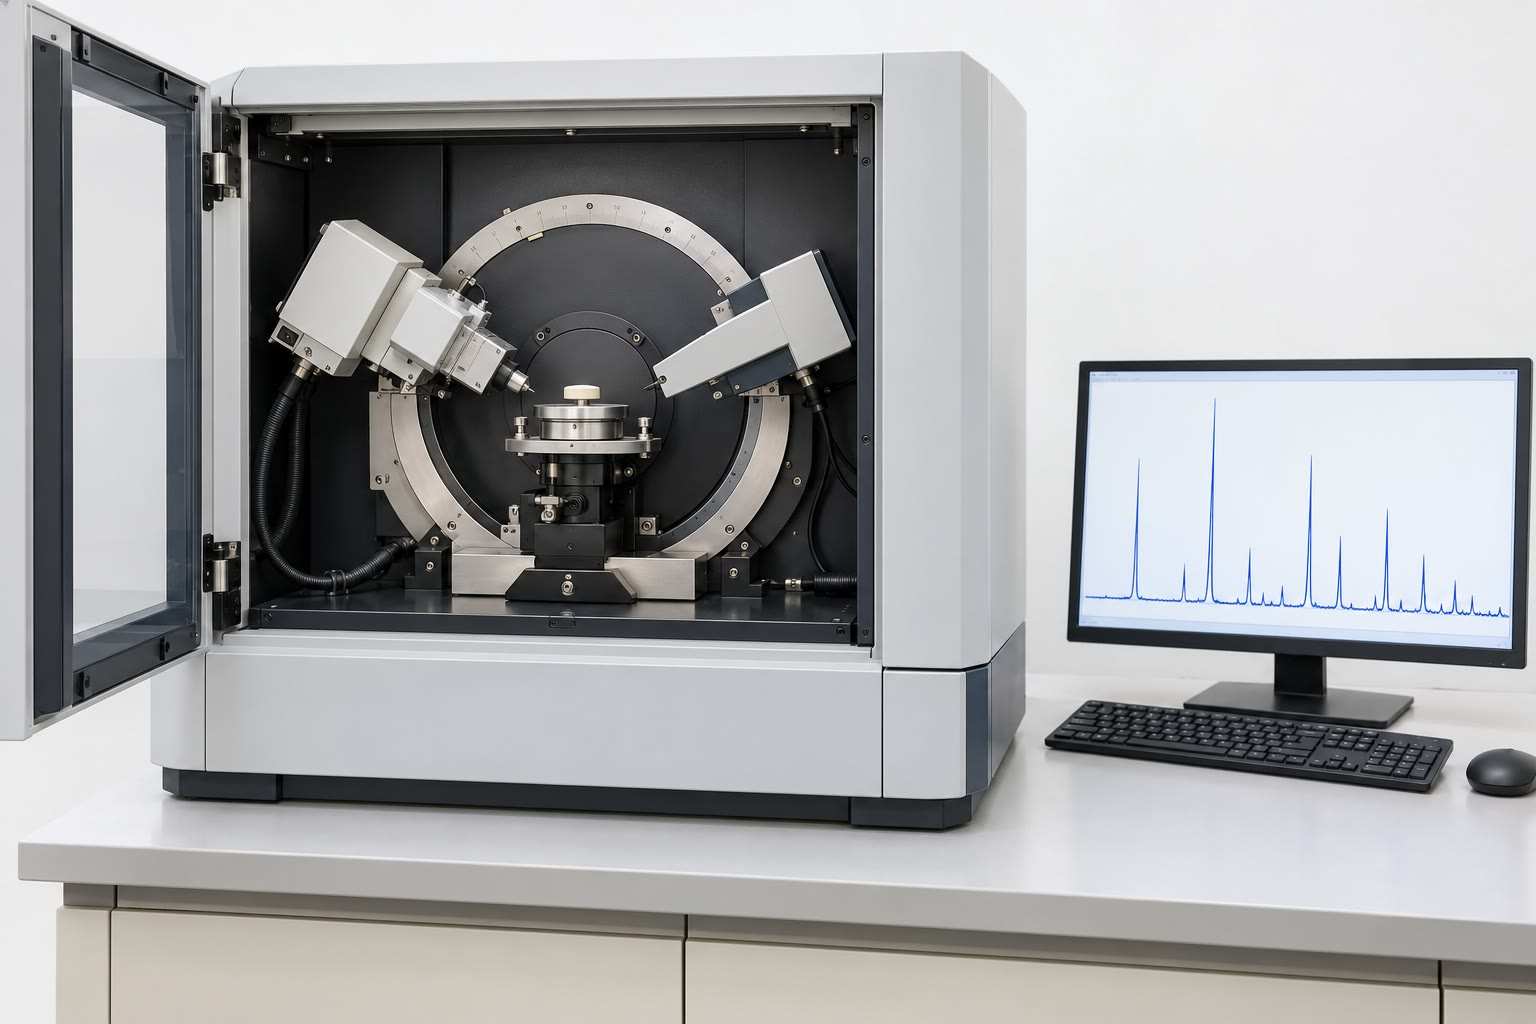
\includegraphics[width=0.6\linewidth]{images/book4/ai/b3-09-diffractometer.jpg}

{\small Difraktometer serbuk meja: tabung sinar-X dan detektornya berputar
pada sebuah lingkaran di sekeliling sampel yang datar.}
\end{omfigure}

\section{Sistem kristal dan kisi Bravais}

Sebuah kisi hanya dapat mempunyai \omterm{def:b3:point-groups:operation}{operasi simetri} yang memetakan kisi itu ke
dirinya sendiri. Hal itu sangat membatasinya.

\begin{theorem}[Pembatasan kristalografis]\label{thm:b3:x-ray-diffraction:restriction}
Satu-satunya sumbu rotasi yang sesuai dengan sebuah kisi adalah sumbu berorde
1, 2, 3, 4, dan 6.
\end{theorem}

\begin{proof}
Dalam basis vektor-vektor kisi, rotasi simetri memetakan vektor kisi ke vektor
kisi, sehingga matriksnya berentri bilangan bulat dan jejaknya bilangan bulat.
Trace itu tidak bergantung pada basis; dalam basis ortonormal dengan $z$
sepanjang sumbu, jejak itu sama dengan $1 + 2\cos\theta$. Jadi $2\cos\theta$
adalah bilangan bulat antara $-2$ dan 2:
$\cos\theta \in \{-1, -\frac12, 0, \frac12, 1\}$, $\theta = 180^\circ, 120^\circ, 90^\circ,
60^\circ, 0^\circ$: orde 2, 3, 4, 6, 1. Sumbu lipat lima mustahil.
\end{proof}

\begin{definition}[Sistem kristal, kisi Bravais, pemusatan kisi]\label{def:b3:x-ray-diffraction:crystal-system}
Menurut simetrinya, kisi-kisi dikelompokkan menjadi tujuh \emph{sistem
kristal}\index{sistem kristal} (triklinik, monoklinik, ortorombik, tetragonal,
trigonal, heksagonal, kubik). Sebuah sel dapat memuat simpul kisi hanya di
sudut-sudutnya (primitif, P) atau juga di pusatnya (berpusat badan, I), di
pusat semua mukanya (berpusat muka, F) atau di pusat sepasang muka (berpusat
alas, C), atau sepanjang sebuah diagonal ruang (rombohedral, R): inilah
\emph{pemusatan kisi}\index{pemusatan kisi} sel itu. Ke-14 kombinasi berbeda
antara sistem dan pemusatan disebut \emph{kisi Bravais}\index{kisi Bravais}.
\end{definition}

\begin{center}\small
\begin{tabular}{lll}
\hline
sistem & batasan sel & pemusatan \\ \hline
triklinik & tidak ada & P \\
monoklinik & $\alpha = \gamma = 90^\circ$ & P, C \\
ortorombik & $\alpha = \beta = \gamma = 90^\circ$ & P, C, I, F \\
tetragonal & $a = b$, semua sudut $90^\circ$ & P, I \\
trigonal & $a = b = c$, $\alpha = \beta = \gamma \ne 90^\circ$ (sumbu rombohedral) & R \\
heksagonal & $a = b$, $\alpha = \beta = 90^\circ$, $\gamma = 120^\circ$ & P \\
kubik & $a = b = c$, semua sudut $90^\circ$ & P, I, F \\ \hline
\end{tabular}
\end{center}

\begin{omfigure}
\tdplotsetmaincoords{60}{100}
\begin{tikzpicture}[tdplot_main_coords, scale=1.25, font=\small]
  \foreach \s/\lab in {0/{kubik P}, 3.0/{kubik I}, 6.0/{kubik F}}{
    \begin{scope}[xshift=\s cm]
      \pic[transform shape] {omcubeo={1.6}};
      \foreach \x in {0,1.6}{\foreach \y in {0,1.6}{\foreach \z in {0,1.6}{\node[cellA=2.6mm] at (\x,\y,\z) {};}}}
      \node[anchor=north] at (0.8,0.8,-0.62) {\lab};
    \end{scope}}
  \begin{scope}[xshift=3.0cm]
    \node[cellB=2.6mm] at (0.8,0.8,0.8) {};
  \end{scope}
  \begin{scope}[xshift=6.0cm]
    \foreach \p in {(0.8,0.8,0),(0.8,0.8,1.6),(0.8,0,0.8),(0.8,1.6,0.8),(0,0.8,0.8),(1.6,0.8,0.8)}{\node[cellB=2.6mm] at \p {};}
  \end{scope}
\end{tikzpicture}

{\small Ketiga \omterm{def:b3:x-ray-diffraction:crystal-system}{kisi Bravais} kubik: primitif (simpul di sudut-sudut), berpusat
badan (ditambah pusat, merah), dan berpusat muka (ditambah keenam pusat muka,
merah). Sel-selnya memuat 1, 2, dan 4 simpul.}
\end{omfigure}

\section{Bidang kisi dan kisi resiprokal}

\begin{definition}[Bidang kisi, indeks Miller, jarak antarbidang]\label{def:b3:x-ray-diffraction:miller}
Yang disebut \emph{bidang kisi}\index{bidang kisi} adalah bidang yang melalui
sedikitnya tiga simpul yang tidak segaris; bidang itu termasuk dalam sebuah
keluarga bidang sejajar yang berjarak sama dan memuat semua simpul. Jika
bidang keluarga itu yang paling dekat dengan titik asal memotong sumbu-sumbu
pada $a/h$, $b/k$, $c/l$, bilangan-bilangan bulat $(hkl)$, tanpa faktor
persekutuan, disebut \emph{indeks Miller}\index{indeks Miller} bidang itu
(indeks 0 untuk bidang yang sejajar dengan sebuah sumbu). Jarak antara
bidang-bidang yang bersebelahan disebut \emph{jarak
antarbidang}\index{jarak antarbidang} $d_{hkl}$.
\end{definition}

\begin{proposition}[Jarak antarbidang dalam sel ortogonal]\label{prop:b3:x-ray-diffraction:spacing}
Untuk sel ortorombik, $\dfrac{1}{d_{hkl}^2} = \dfrac{h^2}{a^2} + \dfrac{k^2}{b^2} +
\dfrac{l^2}{c^2}$; untuk sel kubik, $d_{hkl} = a/\sqrt{h^2 + k^2 + l^2}$.
\end{proposition}

\begin{proof}
Bidang $hx/a + ky/b + lz/c = 1$ mempunyai vektor normal $\mathbf n = (h/a, k/b, l/c)$
dan berjarak $1/|\mathbf n|$ dari titik asal; bidang sejajar yang melalui titik
asal termasuk dalam keluarga itu, sehingga $d = 1/|\mathbf n|$.
\end{proof}

\begin{definition}[Kisi resiprokal]\label{def:b3:x-ray-diffraction:reciprocal}
Untuk kisi dengan vektor-vektor basis $\mathbf a$, $\mathbf b$, $\mathbf c$ dan volume
sel $V$, yang disebut \emph{kisi resiprokal}\index{kisi resiprokal} adalah
kisi dengan vektor-vektor basis
$\mathbf a^* = (\mathbf b\times\mathbf c)/V$, $\mathbf b^* = (\mathbf c\times\mathbf a)/V$,
$\mathbf c^* = (\mathbf a\times\mathbf b)/V$, sehingga $\mathbf a\cdot\mathbf a^* = 1$ dan
$\mathbf a\cdot\mathbf b^* = 0$. Simpulnya $\mathbf G_{hkl} = h\mathbf a^* + k\mathbf b^* + l\mathbf c^*$
tegak lurus pada bidang-bidang $(hkl)$, dan $|\mathbf G_{hkl}| = 1/d_{hkl}$.
\end{definition}

\section{Difraksi}

\begin{theorem}[Hukum Bragg]\label{thm:b3:x-ray-diffraction:bragg}
Sinar-X dengan panjang gelombang $\lambda$ dipantulkan oleh sebuah keluarga
bidang berjarak $d$ hanya pada sudut sapu $\theta$ yang memenuhi
\[
2d\sin\theta = n\lambda, \qquad n = 1, 2, \dots,
\]
yaitu \emph{hukum Bragg}\index{hukum Bragg}. Orde $n$ diserap dengan menuliskan
pantulannya sebagai $(nh\,nk\,nl)$ dengan jarak $d/n$.
\end{theorem}

\begin{proof}
Sinar-sinar yang dihamburkan oleh dua bidang yang bersebelahan, dengan sudut
datang dan sudut pantul yang sama, $\theta$, berselisih lintasan sebesar
$2d\sin\theta$ (kedua ruas di kedua sisi garis normal melalui bidang bawah).
Sinar-sinar itu saling menguatkan jika selisih ini sama dengan bilangan bulat
kali panjang gelombang; dengan jutaan bidang, sudut lain mana pun memberikan
sinar-sinar yang saling meniadakan berpasangan.
\end{proof}

\begin{omfigure}
\begin{tikzpicture}[font=\small, >=Stealth]
  \foreach \y in {0,-1.1}{\draw[thick] (-0.4,\y) -- (7.4,\y);}
  \foreach \x in {0,1.4,...,7.0}{\fill (\x,0) circle (1.5pt) (\x,-1.1) circle (1.5pt);}
  \draw[->, omDef, thick] (0.2,1.75) -- (2.8,0);
  \draw[->, omDef, thick] (2.8,0) -- (5.4,1.75);
  \draw[->, omDef, thick] (-1.43,1.75) -- (2.8,-1.1);
  \draw[->, omDef, thick] (2.8,-1.1) -- (7.03,1.75);
  \draw[densely dashed] (2.8,0) -- (2.8,-1.1);
  \draw[omThm, thick] (2.8,0) -- (2.18,-0.68) (2.8,0) -- (3.42,-0.68);
  \draw[omThm, very thick] (2.18,-0.68) -- (2.8,-1.1) -- (3.42,-0.68);
  \draw (1.8,0) arc[start angle=180, end angle=213.9, radius=1.0];
  \node[anchor=east] at (1.85,-0.2) {$\theta$};
  \draw[<->] (7.7,0) -- (7.7,-1.1) node[midway, right] {$d$};
  \node[omThm, anchor=north] at (2.8,-1.2) {selisih lintasan $2d\sin\theta$};
\end{tikzpicture}

{\small Konstruksi Bragg. Sinar-sinar yang dipantulkan oleh bidang-bidang yang
bersebelahan menempuh jarak lebih jauh sebesar kedua ruas merah, masing-masing
$d\sin\theta$; gelombang-gelombangnya saling menguatkan jika $2d\sin\theta$ sama
dengan bilangan bulat kali panjang gelombang.}
\end{omfigure}

\begin{proposition}[Syarat Laue]\label{prop:b3:x-ray-diffraction:laue}
Dengan vektor gelombang datang dan terhambur $\mathbf k$ dan $\mathbf k'$ yang
panjangnya $1/\lambda$, difraksi terjadi jika $\mathbf k' - \mathbf k = \mathbf G_{hkl}$,
sebuah vektor \omterm{def:b3:x-ray-diffraction:reciprocal}{kisi resiprokal}; syarat ini setara dengan \omterm{thm:b3:x-ray-diffraction:bragg}{hukum Bragg}.
\end{proposition}

\begin{proof}
Gelombang-gelombang yang dihamburkan oleh dua simpul yang dipisahkan oleh
vektor kisi $\mathbf R$ berselisih fase sebesar $2\pi(\mathbf k' - \mathbf k)\cdot\mathbf R$;
semuanya saling menguatkan jika selisih ini kelipatan $2\pi$ untuk setiap
$\mathbf R$, yaitu jika $\mathbf k' - \mathbf k$ berada dalam \omterm{def:b3:x-ray-diffraction:reciprocal}{kisi resiprokal} (menurut
definisi $\mathbf a\cdot\mathbf a^* = 1$, $\mathbf a\cdot\mathbf b^* = 0$\dots). Untuk
hamburan elastis, $|\mathbf k| = |\mathbf k'|$ dan $|\mathbf k' - \mathbf k| = 2\sin\theta/\lambda$,
dengan $2\theta$ sudut di antara keduanya; dengan $|\mathbf G| = 1/d$ syarat ini
menjadi $2d\sin\theta = \lambda$, dan $\mathbf G$ tegak lurus pada bidang-bidang
pemantul.
\end{proof}

\begin{definition}[Bola Ewald]\label{def:b3:x-ray-diffraction:ewald}
Yang disebut \emph{bola Ewald}\index{bola Ewald} adalah bola berjari-jari
$1/\lambda$ yang melalui titik asal \omterm{def:b3:x-ray-diffraction:reciprocal}{kisi resiprokal}, dengan pusatnya pada $-\mathbf k$
dari titik asal; pantulan terjadi setiap kali sebuah simpul \omterm{def:b3:x-ray-diffraction:reciprocal}{kisi resiprokal}
terletak padanya.
\end{definition}

\begin{omfigure}
\begin{tikzpicture}[font=\small, >=Stealth, scale=0.9]
  \foreach \i in {-2,...,4}{\foreach \j in {-2,...,2}{\fill[black!60] (\i*1.0,\j*0.75) circle (1.3pt);}}
  \node[anchor=north east] at (0,0) {$O$};
  \draw[omDef] (-1.625,0.0) circle (1.625);
  \draw[->, omDef, thick] (-1.625,0) -- (0,0) node[midway, below] {$\mathbf k$};
  \draw[->, omThm, thick] (-1.625,0) -- (-1.0,1.5);
  \node[omThm, anchor=east] at (-1.4,0.85) {$\mathbf k'$};
  \draw[->, black, very thick] (0,0) -- (-1.0,1.5) node[pos=0.3, left] {$\mathbf G$};
  \node[anchor=north] at (-1.625,-1.75) {bola Ewald, jari-jari $1/\lambda$};
  \draw[<->] (4.6,0) -- (4.6,0.75) node[midway, right] {$b^*$};
  \draw[<->] (3,-1.85) -- (4,-1.85) node[midway, below] {$a^*$};
\end{tikzpicture}

{\small Konstruksi Ewald dalam dua dimensi (lingkarannya melalui titik asal $O$
\omterm{def:b3:x-ray-diffraction:reciprocal}{kisi resiprokal}). Simpul $\mathbf G$ yang terletak pada lingkaran memberikan
berkas terdifraksi $\mathbf k' = \mathbf k + \mathbf G$. Di sini lingkaran itu, yang
jari-jarinya dipilih untuk keperluan gambar, melalui simpul $(-1, 2)$.}
\end{omfigure}

\section{Intensitas dan simetri}

\omterm{thm:b3:x-ray-diffraction:bragg}{Hukum Bragg} memberikan arah berkas-berkas terdifraksi, yang hanya bergantung
pada kisi; intensitasnya bergantung pada isi sel.

\begin{definition}[Faktor hamburan atom, faktor struktur]\label{def:b3:x-ray-diffraction:structure-factor}
Yang disebut \emph{faktor hamburan atom}\index{faktor hamburan atom} $f_j$
sebuah atom adalah amplitudo yang dihamburkannya, dalam satuan amplitudo satu
elektron; nilainya sama dengan banyaknya elektron atom itu ke arah depan dan
menurun pada sudut yang lebih besar. Yang disebut \emph{faktor
struktur}\index{faktor struktur} pantulan $hkl$ adalah
\[
F_{hkl} = \sum_jf_j\,\eu^{2\pi\iu(hx_j + ky_j + lz_j)},
\]
yang dijumlahkan atas atom-atom sel pada koordinat pecahan $(x_j, y_j, z_j)$.
\end{definition}

\begin{proposition}[Intensitas]\label{prop:b3:x-ray-diffraction:intensity}
Intensitas sebuah pantulan sebanding dengan $|F_{hkl}|^2$.
\end{proposition}

\begin{proof}[Bukti parsial]
Atom $j$ terletak pada $\mathbf r_j = x_j\mathbf a + y_j\mathbf b + z_j\mathbf c$; untuk sebuah
pantulan, $(\mathbf k' - \mathbf k)\cdot\mathbf r_j = hx_j + ky_j + lz_j$, sehingga
gelombangnya mempunyai fase $2\pi(hx_j + ky_j + lz_j)$ relatif terhadap atom di
titik asal, dan amplitudo $f_j$: sel itu menghamburkan jumlah $F_{hkl}$, dan
setiap sel menghamburkan hal yang sama. Intensitas adalah kuadrat modulus
amplitudo. Bahwa hamburan berganda dapat diabaikan (pendekatan kinematik)
diterima tanpa bukti.
\end{proof}

\begin{definition}[Ketakhadiran sistematis]\label{def:b3:x-ray-diffraction:absence}
Yang disebut \emph{ketakhadiran sistematis}\index{ketakhadiran sistematis}
adalah pantulan yang \omterm{def:b3:x-ray-diffraction:structure-factor}{faktor strukturnya} lenyap untuk setiap kristal dengan
\omterm{def:b3:x-ray-diffraction:crystal-system}{pemusatan kisi} atau simetri tertentu, apa pun atom-atomnya.
\end{definition}

\begin{proposition}[Ketakhadiran pada kisi berpusat]\label{prop:b3:x-ray-diffraction:absences}
Dalam kisi berpusat badan, pantulan dengan $h + k + l$ ganjil tidak hadir;
dalam kisi berpusat muka, pantulan dengan $h$, $k$, $l$ berparitas campuran
tidak hadir.
\end{proposition}

\begin{proof}
Pemusatan I: setiap atom pada $(x,y,z)$ mempunyai salinan pada
$(x + \frac12, y + \frac12, z + \frac12)$, yang faktor fasenya berbeda sebesar
$\eu^{\iu\pi(h+k+l)} = (-1)^{h+k+l}$: $F = (1 +
(-1)^{h+k+l})F'$. Pemusatan F: salinan-salinan pada tiga pusat muka memberikan
faktor $1 +
(-1)^{h+k} + (-1)^{h+l} + (-1)^{k+l}$, yang sama dengan 4 jika $h$, $k$, $l$
semuanya genap atau semuanya ganjil, dan 0 jika tidak.
\end{proof}

\begin{example}[Garam batu dan silvit]\label{ex:b3:x-ray-diffraction:nacl-kcl}
% ledger: lat:NaCl, lat:KCl
Dalam struktur garam batu, kation pada $(0,0,0)$ dan anion pada $(\frac12,0,0)$,
masing-masing dengan translasi F: $F_{hkl} = 4[f_+ + f_-(-1)^{h+k+l}]$ untuk
indeks yang tidak campuran. Untuk \ce{NaCl}, $f(\ce{Na+}) \approx 10$ dan
$f(\ce{Cl-}) \approx 18$: pantulan-pantulan yang semua indeksnya ganjil, (111) dan
(311), lemah tetapi hadir. Untuk \ce{KCl}, \ce{K+} dan \ce{Cl-} sama-sama
mempunyai 18 elektron: pantulan-pantulan yang semua indeksnya ganjil hampir
lenyap, dan polanya tampak seperti pola kisi kubik primitif dengan rusuk sel
setengahnya (gambar di bawah).
\end{example}

\begin{omfigure}
\begin{tikzpicture}
\begin{axis}[name=salts, width=0.95\linewidth, height=5.2cm, xmin=20, xmax=90,
  ymin=0, ymax=2.55, ytick=\empty, axis x line=bottom, axis y line=none,
  xlabel={$2\theta$ / derajat (Cu K$\alpha_1$)}, tick label style={font=\small},
  label style={font=\small}]
\addplot[omDef, thin] table[x=tt, y expr=\thisrow{NaCl}+1.35] {figdata/out/bachelor-3-xrd-powder-salts.dat};
\addplot[omThm, thin] table[x=tt, y=KCl] {figdata/out/bachelor-3-xrd-powder-salts.dat};
\node[font=\small, omDef, anchor=west] at (axis cs:79,1.9) {\ce{NaCl}};
\node[font=\small, omThm, anchor=west] at (axis cs:77,0.55) {\ce{KCl}};
\node[font=\scriptsize, anchor=south] at (axis cs:27.36,1.52) {111};
\node[font=\scriptsize, anchor=west] at (axis cs:32.1,2.25) {200};
\node[font=\scriptsize, anchor=west] at (axis cs:28.8,0.9) {200};
\node[font=\scriptsize, anchor=west] at (axis cs:41.0,0.85) {220};
\end{axis}
\end{tikzpicture}

\begin{tikzpicture}
\begin{axis}[name=met, width=0.62\linewidth, height=4.4cm, xmin=35, xmax=100,
  ymin=0, ymax=2.35, ytick=\empty, axis x line=bottom, axis y line=none,
  xlabel={$2\theta$ / derajat}, tick label style={font=\small}, label style={font=\small}]
\addplot[omDef, thin] table[x=tt, y expr=\thisrow{Cu}+1.2] {figdata/out/bachelor-3-xrd-powder-metals.dat};
\addplot[omThm, thin] table[x=tt, y=W] {figdata/out/bachelor-3-xrd-powder-metals.dat};
\node[font=\small, omDef, anchor=west] at (axis cs:55,1.5) {Cu (F)};
\node[font=\small, omThm, anchor=west] at (axis cs:44,0.4) {W (I)};
\end{axis}
\begin{axis}[at={(met.east)}, anchor=west, xshift=0.7cm, width=0.36\linewidth, height=4.4cm,
  xmin=29.7, xmax=33.7, ymin=0, ymax=1.1, ytick=\empty, axis x line=bottom,
  axis y line=none, xlabel={$2\theta$ / derajat}, tick label style={font=\small},
  label style={font=\small}, title={\small Scherrer}]
\addplot[black, thick] table[x=tt, y=L200] {figdata/out/bachelor-3-xrd-powder-scherrer.dat};
\addplot[omDef, thick] table[x=tt, y=L50] {figdata/out/bachelor-3-xrd-powder-scherrer.dat};
\addplot[omThm, thick] table[x=tt, y=L10] {figdata/out/bachelor-3-xrd-powder-scherrer.dat};
\end{axis}
\end{tikzpicture}

{\small Pola serbuk hasil perhitungan (Cu K$\alpha_1$; faktor hamburan dianggap
sama dengan banyaknya elektron, sehingga hanya ketakhadiran dan kecenderungan
umum intensitas yang bermakna). Atas: \ce{NaCl} dan \ce{KCl}; garis-garis
\ce{KCl} yang semua indeksnya ganjil lenyap. Kiri bawah: tembaga (F)
memperlihatkan (111), (200), (220), (311)\dots; tungsten (I) memperlihatkan
(110), (200), (211)\dots. Kanan bawah: garis (200) \ce{NaCl} untuk kristalit
berukuran 200 (hitam), 50 (biru), dan 10 nm (merah): kristal yang lebih kecil
memberikan garis yang lebih lebar.}
\end{omfigure}

\begin{proposition}[Hukum Friedel]\label{prop:b3:x-ray-diffraction:friedel}
Tanpa hamburan anomali, $|F_{hkl}| = |F_{\bar h\bar k\bar l}|$: pola difraksi
tampak sentrosimetris meskipun kristalnya tidak.
\end{proposition}

\begin{proof}
Dengan $f_j$ real, $F_{\bar h\bar k\bar l} = \sum f_j\eu^{-2\pi\iu(\dots)} = F_{hkl}^*$,
yang modulusnya sama.
\end{proof}

\omterm{def:b3:point-groups:operation}{Unsur-unsur simetri} yang menggabungkan rotasi atau pencerminan dengan
sebagian translasi kisi hanya ada dalam kristal.

\begin{definition}[Sumbu ulir, bidang luncur, grup ruang]\label{def:b3:x-ray-diffraction:space-group}
Yang disebut \emph{sumbu ulir}\index{sumbu ulir} $n_p$ adalah unsur yang
menggabungkan rotasi sebesar $2\pi/n$ dengan translasi sebesar $p/n$ ulangan
kisi sepanjang sumbu itu ($2_1$: setengah putaran dan setengah sel). Yang
disebut \emph{bidang luncur}\index{bidang luncur} adalah unsur yang
menggabungkan pencerminan dengan translasi sebesar setengah vektor kisi yang
sejajar dengan bidang itu (luncuran $a$, $b$, $c$). Grup semua \omterm{def:b3:point-groups:operation}{operasi simetri}
sebuah kristal, termasuk translasi, disebut \emph{grup ruang}\index{grup ruang}
kristal itu: jumlahnya ada 230. Bagian terkecilnya yang darinya seluruh
kristal dibangkitkan oleh operasi-operasi itu disebut \emph{satuan
asimetris}\index{satuan asimetris}. Himpunan titik yang dibiarkan tetap oleh
sebuah \omterm{def:b3:point-groups:class}{subgrup} operasi disebut \emph{posisi Wyckoff}\index{posisi Wyckoff}:
posisi umum tidak mempunyai simetri, posisi khusus terletak pada \omterm{def:b3:point-groups:operation}{unsur-unsur
simetri}.
\end{definition}

\begin{proposition}[Ketakhadiran akibat sumbu ulir]\label{prop:b3:x-ray-diffraction:screw-absence}
Sumbu $2_1$ sepanjang $b$ membuat pantulan $0k0$ dengan $k$ ganjil tidak hadir.
\end{proposition}

\begin{proof}
Sumbu itu memetakan $(x, y, z)$ ke $(-x, y + \frac12, -z)$. Untuk $h = l = 0$ kedua
atom mempunyai faktor fase $\eu^{2\pi\iu ky}$ dan
$\eu^{2\pi\iu k(y + 1/2)} = (-1)^k\eu^{2\pi\iu ky}$: jumlahnya lenyap untuk $k$
ganjil.
\end{proof}

\begin{method}[Membaca simbol grup ruang]\label{met:b3:x-ray-diffraction:read-space-group}
\begin{enumerate}
  \item Huruf pertama adalah \omterm{def:b3:x-ray-diffraction:crystal-system}{pemusatan kisinya} (P, I, F, C, R).
  \item Simbol-simbol berikutnya memberikan simetri sepanjang arah-arah utama;
        untuk sistem monoklinik, satu-satunya arah itu adalah $b$. Garis
        pecahan berarti ``dengan sebuah bidang yang tegak lurus pada sumbu
        ini''.
  \item \textit{P}$2_1/c$, \omterm{def:b3:x-ray-diffraction:space-group}{grup ruang} yang paling umum bagi molekul organik:
        primitif, sumbu $2_1$ sepanjang $b$, dan \omterm{def:b3:x-ray-diffraction:space-group}{bidang luncur} $c$ yang tegak
        lurus padanya; keduanya membangkitkan \omterm{def:b3:point-groups:inversion}{pusat-pusat inversi}.
        Ketakhadiran: $0k0$ dengan $k$ ganjil, $h0l$ dengan $l$ ganjil.
\end{enumerate}
\end{method}

\begin{omfigure}
\begin{tikzpicture}[x=3.6cm, y=3.6cm, font=\small]
  \draw (0,0) rectangle (1,1);
  \node[anchor=north] at (0.5,-0.05) {$a \rightarrow$};
  \node[anchor=east] at (-0.05,0.5) {$b \uparrow$};
  % c-glide planes perpendicular to b at y = 1/4 and 3/4 (glide along c, normal to the page): dotted
  \draw[black, line width=1.1pt, dotted] (0,0.25) -- (1,0.25) (0,0.75) -- (1,0.75);
  % 2_1 axes parallel to b at x = 0, 1/2, 1 (height z = 1/4): lines with half-arrowheads
  \foreach \x in {0,0.5,1}{
    \draw[black, line width=1pt, {Straight Barb[left]}-{Straight Barb[left]}] (\x,0.03) -- (\x,0.97);}
  \node[font=\scriptsize, anchor=west] at (0.51,0.88) {$\tfrac14$};
  % centres of inversion at the corners, edge midpoints and centre
  \foreach \p in {(0,0),(0.5,0),(1,0),(0,0.5),(0.5,0.5),(1,0.5),(0,1),(0.5,1),(1,1)}{\pic at \p {ominv};}
  % general positions: (x,y,z), (-x,y+1/2,1/2-z), (-x,-y,-z), (x,1/2-y,1/2+z)
  \pic at (0.20,0.10) {omgenpos={$+$}{0}};
  \pic at (0.80,0.60) {omgenpos={$\tfrac12{-}$}{0}};
  \pic at (0.80,0.90) {omgenpos={$-$}{1}};
  \pic at (0.20,0.40) {omgenpos={$\tfrac12{+}$}{1}};
\end{tikzpicture}

{\small \omterm{def:b3:x-ray-diffraction:space-group}{Grup ruang} \textit{P}$2_1/c$ dilihat sepanjang $c$ (proyeksi pada bidang
$ab$). Garis titik-titik: \omterm{def:b3:x-ray-diffraction:space-group}{bidang luncur} $c$ yang tegak lurus pada $b$;
setengah panah: \omterm{def:b3:x-ray-diffraction:space-group}{sumbu ulir} $2_1$ sepanjang $b$ (pada ketinggian $z = \frac14$);
lingkaran kecil: \omterm{def:b3:point-groups:inversion}{pusat inversi}. Sebuah posisi umum pada ketinggian $+z$
membangkitkan tiga posisi lain; tanda koma menandai salinan bayangan cermin
(yang dihasilkan oleh luncuran atau inversi); $\frac12{-}$ berarti ketinggian
$\frac12 - z$.}
\end{omfigure}

\section{Metode serbuk dan metode kristal tunggal}

\begin{definition}[Pola difraksi serbuk]\label{def:b3:x-ray-diffraction:powder}
Sampel yang digerus halus mengandung kristalit dengan segala orientasi: setiap
keluarga bidang menemukan sebagian kristalit dalam posisi memantul, dan
berkas-berkas terdifraksi membentuk kerucut. Intensitas yang direkam terhadap
$2\theta$ disebut \emph{pola difraksi serbuk}\index{pola difraksi serbuk}
sampel itu, sidik jari fase kristalnya.
\end{definition}

\begin{method}[Mengindeks pola serbuk kubik]\label{met:b3:x-ray-diffraction:index-cubic}
\begin{enumerate}
  \item Hitunglah $\sin^2\theta$ untuk setiap garis; untuk kristal kubik
        $\sin^2\theta =
        (\lambda^2/4a^2)N$ dengan $N = h^2 + k^2 + l^2$.
  \item Bagilah dengan nilai terkecil dan carilah deret bilangan bulatnya: P
        memberikan $N = 1, 2, 3, 4, 5, 6, 8, \dots$ (tidak pernah 7); I
        memberikan $2, 4, 6, 8, 10, \dots$; F memberikan
        $3, 4, 8, 11, 12, 16, \dots$
  \item Pilihlah deret yang cocok untuk semua garis; lalu
        $a = \lambda\sqrt N/(2\sin\theta)$, sebaiknya dari garis bersudut besar,
        tempat galat pada $\theta$ paling kecil pengaruhnya.
\end{enumerate}
\end{method}

\begin{method}[Banyaknya satuan rumus dalam sel]\label{met:b3:x-ray-diffraction:z-from-density}
Dengan massa molar $M$ satu satuan rumus dan massa jenis terukur $\rho$, nilai
$Z =
\rho N_Aa^3/M$ (untuk sel kubik) harus berupa bilangan bulat; nilai itu
menguji struktur yang diusulkan.
\end{method}

\begin{proposition}[Persamaan Scherrer]\label{prop:b3:x-ray-diffraction:scherrer}
Kristalit berukuran rata-rata $L$ melebarkan sebuah garis sebesar
$\beta \approx K\lambda/(L\cos\theta)$ (lebar penuh pada setengah maksimum dalam
radian $2\theta$, $K \approx 0.9$).
\end{proposition}
\admitted

Di bawah sekitar \qty{100}{nm} pelebaran itu menjadi terukur; persamaan
Scherrer, yang diturunkan dalam kuliah yang lebih lanjut dari transformasi
Fourier tumpukan bidang yang berhingga, lalu memperkirakan ukuran nanokristal
(\cref{ch:b3:inorganic-materials}).

\begin{definition}[Masalah fase, faktor R]\label{def:b3:x-ray-diffraction:refinement}
Intensitas memberikan $|F_{hkl}|$ tetapi tidak memberikan fase $F_{hkl}$; tanpa
fase itu, \omterm{def:b3:computational-chemistry:dft}{kerapatan elektron} tidak dapat dihitung dengan membalik deret
Fourier. Inilah \emph{masalah fase}\index{masalah fase}. Sebuah struktur coba
dihaluskan dengan kuadrat terkecil sampai modulus hasil perhitungan dan
modulus teramati sesuai; sisaan $R = \sum\big||F_o| - |F_c|\big|/\sum|F_o|$
disebut \emph{faktor R}\index{faktor R} struktur itu --- beberapa persen untuk
struktur yang baik.
\end{definition}

Untuk kristal tunggal, sebuah difraktometer mengukur ribuan pantulan;
metode langsung (hubungan statistik antara fase-fase pantulan yang kuat)
memberikan peta \omterm{def:b3:computational-chemistry:dft}{kerapatan elektron} pertama untuk sebagian besar molekul
kecil, dan penghalusan menempatkan setiap atom sampai beberapa perseribu
nanometer. Hasilnya disimpan sebagai berkas CIF dalam basis data terbuka,
yang menjadi sumber parameter kisi yang dikutip dalam seri ini.

\begin{inthelab}[Pengukuran serbuk]
Serbuk digerus dalam lumpang akik, ditekan rata ke dalam wadah, lalu dipindai
dari 5 sampai \ang{90} dalam $2\theta$ dengan radiasi Cu K$\alpha$; filter nikel
menyingkirkan sebagian besar garis K$\beta$. Polanya dibandingkan dengan
pola-pola acuan dari sebuah basis data, dan parameter kisi dihaluskan dengan
standar internal seperti serbuk silikon. Instrumen sinar-X tertutup dan
berpengaman: penutup berkas tidak dapat terbuka selama pintunya terbuka.
\end{inthelab}

\begin{history}[Keluarga Bragg, 1913]
\begin{minipage}[t]{0.72\linewidth}
Max von Laue mengusulkan pada tahun 1912 bahwa kristal mendifraksikan sinar-X,
dan Walter Friedrich serta Paul Knipping merekam pola yang pertama. William
Lawrence Bragg, yang berusia dua puluh dua tahun, menjelaskan bintik-bintik
itu sebagai pantulan dari \omterm{def:b3:x-ray-diffraction:miller}{bidang-bidang kisi} dan, bersama ayahnya William
Henry Bragg, yang membangun spektrometer sinar-X, memecahkan struktur
\ce{NaCl}, \ce{KCl} dan intan pada tahun 1913. Ayah dan anak itu berbagi Hadiah
Nobel Fisika 1915.
\end{minipage}\hfill
\begin{minipage}[t]{0.22\linewidth}\vspace{0pt}
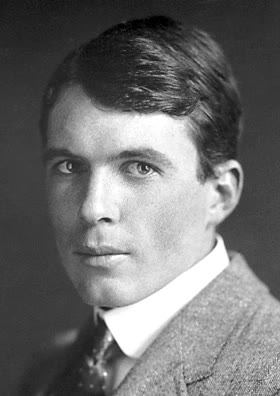
\includegraphics[width=\linewidth]{images/book4/bragg-wl.jpg}\par
{\footnotesize W. L. Bragg.}
\end{minipage}
\end{history}

\section{Latihan}

\begin{exercise}[$\star$]\label{exo:b3:x-ray-diffraction:1}
% ledger: lat:NaCl
Untuk \ce{NaCl} ($a = \qty{564.06}{pm}$), hitunglah $d_{111}$, $d_{200}$ dan $d_{220}$.
\end{exercise}

\begin{exercise}[$\star$]\label{exo:b3:x-ray-diffraction:2}
% ledger: lat:Cu, xray:CuKa1
Tembaga berstruktur FCC dengan $a = \qty{361.50}{pm}$. Dengan Cu K$\alpha_1$
($\lambda = \qty{154.06}{pm}$), hitunglah $2\theta$ kedua pantulan pertamanya,
setelah menamainya.
\end{exercise}

\begin{exercise}[$\star$]\label{exo:b3:x-ray-diffraction:3}
Manakah di antara pantulan 100, 110, 111, 200, 210, 211, 220 yang hadir untuk
kisi kubik P, I, dan F?
\end{exercise}

\begin{exercise}[$\star$]\label{exo:b3:x-ray-diffraction:4}
Berikan basis resiprokal kisi persegi panjang dua dimensi bersisi $a$ dan $b$,
lalu gambarlah simpul-simpul resiprokal yang pertama.
\end{exercise}

\begin{exercise}[$\star\star$]\label{exo:b3:x-ray-diffraction:5}
% ledger: lat:W
Sebuah logam memberikan garis-garis pada $2\theta = 40.27$, 58.26, 73.20, 87.01 dan
\ang{100.66} dengan Cu K$\alpha_1$. Indekslah pola itu, lalu carilah tipe kisi
dan $a$-nya.
\end{exercise}

\begin{exercise}[$\star\star$]\label{exo:b3:x-ray-diffraction:6}
% ledger: lat:KCl
Sebuah kristal \ce{KCl} ($a = \qty{629.29}{pm}$) mempunyai massa jenis terukur
\qty{1.99}{g/cm^3} (data latihan). Carilah $Z$.
\end{exercise}

\begin{exercise}[$\star\star$]\label{exo:b3:x-ray-diffraction:7}
Garis (200) serbuk nano \ce{NaCl} ($2\theta = \ang{31.70}$) selebar \ang{0.40},
dengan instrumen tidak menyumbang apa pun. Perkirakan ukuran kristalitnya.
\end{exercise}

\begin{exercise}[$\star\star$]\label{exo:b3:x-ray-diffraction:8}
\ce{CsCl} mempunyai \ce{Cs+} pada $(0,0,0)$ dan \ce{Cl-} pada $(\frac12,\frac12,\frac12)$
dalam sel P. Dengan $f
\approx$ banyaknya elektron, hitunglah $F_{100}$ dan $F_{110}$ serta rasio
intensitasnya (hanya \omterm{def:b3:x-ray-diffraction:structure-factor}{faktor strukturnya}). Mengapa \ce{CsCl} bukan kisi
berpusat badan?
\end{exercise}

\begin{exercise}[$\star\star$]\label{exo:b3:x-ray-diffraction:9}
Tunjukkan bahwa kisi berpusat C (simpul tambahan pada $(\frac12,\frac12,0)$)
membuat pantulan-pantulan dengan $h + k$ ganjil tidak hadir.
\end{exercise}

\begin{exercise}[$\star\star\star$]\label{exo:b3:x-ray-diffraction:10}
Jelaskan mengapa penemuan pada tahun 1980-an tentang paduan logam yang pola
difraksinya memperlihatkan bintik-bintik tajam dengan simetri lipat sepuluh
tidak bertentangan dengan pembatasan kristalografis, dan apa yang diubahnya
dalam definisi kristal.
\end{exercise}

\begin{exercise}[$\star\star\star$]\label{exo:b3:x-ray-diffraction:11}
Tunjukkan bahwa dalam \textit{P}$2_1/c$ \omterm{def:b3:x-ray-diffraction:space-group}{bidang luncur} membuat pantulan $h0l$
dengan $l$ ganjil tidak hadir.
\end{exercise}

\begin{exercise}[$\star\star\star$]\label{exo:b3:x-ray-diffraction:12}
Sebuah enantiomer murni tidak pernah dapat mengkristal dalam \omterm{def:b3:x-ray-diffraction:space-group}{grup ruang} yang
memuat \omterm{def:b3:point-groups:inversion}{pusat inversi}, cermin, atau \omterm{def:b3:x-ray-diffraction:space-group}{bidang luncur}. Mengapa? Pada jenis \omterm{def:b3:x-ray-diffraction:space-group}{grup
ruang} apa enantiomer itu terbatas, dan apa yang tersirat dari hukum Friedel
bagi penentuan konfigurasi absolutnya?
\end{exercise}
% tahan judul bersama kotak soalnya, yang memenuhi satu halaman sendiri
% keep the heading with its problem box, which fills a page by itself
\clearpage
\enlargethispage{3\baselineskip}
\section{Soal: Serbuk Putih yang Mana?}

\begin{problem}[{Soal akhir pekan --- pola serbuk sebuah garam kubik yang tidak
diketahui: jarak antarbidang, pengindeksan, parameter kisi dan identitas
garam itu, serta ukuran kristalitnya}]
\label{pb:b3:x-ray-diffraction:1}
% ledger: xray:CuKa1, lat:NaCl, lat:KCl, lat:KBr
Sebuah serbuk kristal putih yang belum dikenal, entah \ce{NaCl}, \ce{KCl}
atau \ce{KBr}, memberikan garis-garis ini dengan radiasi Cu K$\alpha_1$
($\lambda = \qty{154.059}{pm}$; data soal, dihitung untuk latihan ini):
\begin{center}\small
\begin{tabular}{lcccccc}
\hline
$2\theta$ / derajat & 28.342 & 40.512 & 50.178 & 58.632 & 66.380 & 73.692 \\
intensitas relatif & 100 & 92 & 38 & 20 & 61 & 49 \\ \hline
\end{tabular}
\end{center}
Tidak ada garis lain yang muncul antara 20 dan \ang{75}. Parameter kisi acuan:
\ce{NaCl} \qty{564.06}{pm}, \ce{KCl} \qty{629.29}{pm}, \ce{KBr} \qty{658.47}{pm}.
Massa molar: K 39.1, Na 23.0, Cl 35.5, Br \qty{79.9}{g/mol}.

\medskip\noindent\textbf{Bagian I --- \omterm{def:b3:x-ray-diffraction:miller}{Jarak antarbidang}.}
\begin{enumerate}[beginpenalty=10000]
  \item Hitunglah $\theta$ dan $d$ untuk garis pertama.
  \item Hitunglah $d$ untuk semua garis.
  \item Hitunglah rasio-rasio $\sin^2\theta/\sin^2\theta_1$.
  \item Deret bilangan bulat apa yang diperoleh?
  \item Mungkinkah pola itu milik kisi kubik primitif? Dengan $a$ berapa?
  \item Untuk kisi kubik primitif, bilangan bulat $N$ mana yang tidak pernah
        muncul? Apakah sejauh ini pola itu dapat membedakan kedua tafsiran?
\end{enumerate}

\medskip\noindent\textbf{Bagian II --- Kisi yang sebenarnya.}
\begin{enumerate}[resume, beginpenalty=10000]
  \item Ketiga kandidat merupakan kisi F. Indekslah garis-garisnya dengan
        deret F.
  \item Simpulkan $a$ dari garis pertama.
  \item Kandidat mana yang cocok?
  \item Untuk garam itu, mengapa pantulan-pantulan yang semua indeksnya ganjil,
        (111) dan (311), tidak hadir?
  \item Apakah \ce{NaCl} akan memperlihatkan (111)? Dan \ce{KBr}?
  \item Jelaskan mengapa tafsiran primitif pada Bagian I merupakan jebakan.
\end{enumerate}

\medskip\noindent\textbf{Bagian III --- Massa jenis dan isi sel.}
\begin{enumerate}[resume, beginpenalty=10000]
  \item Berapa satuan rumus yang dimuat sel itu?
  \item Hitunglah massa jenis dari sel itu.
  \item Berikan bilangan koordinasi setiap ion.
  \item Hitunglah jarak K--Cl yang terpendek.
  \item Pantulan apa yang akan muncul pertama di atas \ang{75}?
  \item Mengapa intensitas kurang berguna daripada posisi untuk
        mengidentifikasi sebuah fase?
\end{enumerate}

\medskip\noindent\textbf{Bagian IV --- Penghalusan dan ukuran kristalit.}
\begin{enumerate}[resume, beginpenalty=10000]
  \item Mengapa parameter kisi paling baik dihitung dari garis bersudut besar?
  \item Hitunglah $a$ dari garis (420).
  \item Garis (420) selebar \ang{0.25} dalam $2\theta$ (lebar instrumental dapat
        diabaikan). Perkirakan ukuran kristalitnya.
  \item Apakah ukuran kristalit \qty{1}{\micro m} akan melebarkan garis itu
        secara terukur?
  \item Nyatakan hasilnya: parameter kisi yang dihaluskan dari garis (420)
        dan identitas serbuk.
\end{enumerate}
\end{problem}
